
Now that we have cleaned our single detector triggers SNR distribution we want to assess the significance of the triggers, especially for those in the tail of the distribution since this is where we expect to find astrophysical events.
The ranking statistics tells us how loud an event was.
It is only relevant when comparing MBTA triggers with each other and does not tell whether a trigger is likely to be of astrophysical origin or not.
This selection, for sending public alerts, is instead done using the False Alarm Rate (FAR) described in \ref{sec:far_coinc}.
This chapter describes several option for the single detector triggers FAR computation.


\subsection{Extrapolating the observed background}

To compute a FAR for the single detector triggers, a first possibility is to extrapolate the observed O3 background.
In chapter \ref{section:selection} we have shown that we can significantly reduce the background for EM bright single detector triggers.
This allows to remove the tails of the distribution.
The remaining background rwSNR distribution is then close to an exponential distribution.
We can therefore fit the distribution using an exponential function to reach lower rates for background events which can be used to assign lower FAR values to high rwSNR candidates.
Figure \ref{fig:fitO3} shows such a fit on O3 EM bright single detector triggers after aplying the selection criteria.
The fitting function is $\textrm{FAR$_{8.6}$} \times \exp(\textrm{slope} \times (\textrm{rwSNR}-8.6))$, such that ``FAR$_{8.6}$'' is the cumulative background rate (equal to the FAR) at rwSNR$=8.6$.
This choice is made in order to reduce a bit the correlation between the parameters of the fit.
Two fits are performed.
One on the tail of the distribution only ($8.4<\text{rwSNR}<9.1$) and the other on the full distribution.
Results of the fits are reported in table \ref{tab:fitO3}.
The errors on the cumulative rate were adjusted to have a $\chi^2/$NDF close to 1 in order to have a reasonable estimate of the errors on the fit.

\begin{table}[h]
  \centering
  \resizebox{\linewidth}{!}{%
  \begin{tabular}{c|c|c|c|c|c|c}
    %Detector & fit range & FAR$_8$ (days$^{-1}$) & slope & $\chi^2/$NDF & IFAR$_9$ (days) & IFAR$_{10}$ (years) \\ \hline
    %H1 & [8.4, 9.1] & 2.0 $\pm$ 2.3 & -7.9 $\pm$ 2.1 & 0.1 & 7.16e-04 $\pm$ 2.82e-03 & 2.56e-7 $\pm$ 3.07e-6 \\ \hline
    %H1 & [8.0, 9.1] & 1.2 $\pm$ 0.1 & -6.9 $\pm$ 0.3 & 0.3 & 1.21e-03 $\pm$ 1.35e-03 & 1.19e-06 +/- 2.86e-06 \\ \hline
    %L1 & [8.4, 9.1] & 0.5 $\pm$ 0.6 & -5.2 $\pm$ 1.8 & 0.5 & 2.88e-03 $\pm$ 8.76e-03 & 1.59e-5 $\pm$ 1.59e-4 \\ \hline
    %L1 & [8.0, 9.1] & 1.2 $\pm$ 0.1 & -6.8 $\pm$ 0.3 & 0.4 & 1.46e-03 $\pm$ 1.64e-03 & 1.71e-6 $\pm$ 4.15e-6 \\ 
    %
    %H1 & [8.0, 9.1] & 1.2 $\pm$ 0.1 & -6.9 $\pm$ 0.3 & 0.3 & 829.27 $\pm$ 927.2 & 2305.3 $\pm$ 5542.5 \\ \hline
    %L1 & [8.0, 9.1] & 1.2 $\pm$ 0.1 & -6.8 $\pm$ 0.3 & 0.4 & 686.26 $\pm$ 770.2 & 1601.0 $\pm$ 3878.4 \\ 
    %H1 & [8.4, 9.1] & 2.0 $\pm$ 2.3 & -7.9 $\pm$ 2.1 & 0.1 & 1397.02 $\pm$ 5509.8 & 10694.9 $\pm$ 128363.8 \\ \hline
    %L1 & [8.4, 9.1] & 0.5 $\pm$ 0.6 & -5.2 $\pm$ 1.8 & 0.5 & 347.75 $\pm$ 1050.0 & 172.5 $\pm$ 1726.8 \\ \hline
    %
    Detector & fit range & FAR$_{8.6}$ (days$^{-1}$) & slope & IFAR$_8$ (days) & IFAR$_9$ (years) & IFAR$_{10}$ (centuries) \\ \hline
    H1 & [8.0, 9.1] & 0.019 $\pm$ 0.002 & -6.9 $\pm$ 0.2 & 0.8 $\pm$ 0.03 & 2.3 $\pm$ 0.3 & 23.1 $\pm$ 7.2 \\ \hline
    L1 & [8.0, 9.1] & 0.022 $\pm$ 0.002 & -6.8 $\pm$ 0.2 & 0.8 $\pm$ 0.04 & 1.9 $\pm$ 0.4 & 16.0 $\pm$ 6.4 \\ \hline
    H1 & [8.4, 9.1] & 0.017 $\pm$ 0.001 & -7.9 $\pm$ 0.6 & 0.5 $\pm$ 0.2 & 3.8 $\pm$ 1.2 & 107 $\pm$ 100 \\ \hline
    L1 & [8.4, 9.1] & 0.023 $\pm$ 0.003 & -5.2 $\pm$ 1.3 & 1.9 $\pm$ 1.4 & 1.0 $\pm$ 0.5 & 1.7 $\pm$ 3.1 \\ \hline

  \end{tabular}}
  \caption{Fit parameters obtained on O3 EM bright single detector triggers after selection criteria.}
  \label{tab:fitO3}
\end{table}

\begin{figure}
  \centering
  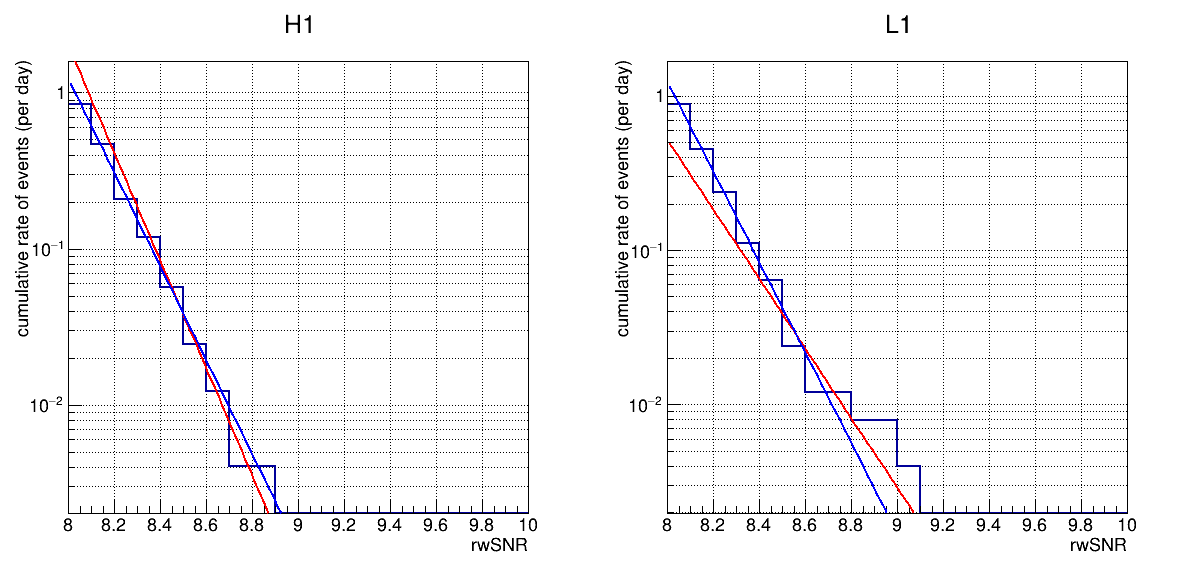
\includegraphics[width=\linewidth]{sectionFAR/simpleFit/cSimpleFitO3.png}
  \caption{rwSNR distribution of O3 EM bright single detector triggers after selection with an exponential fit. The red curves are fitted on [8.4, 9.1]. The blue curves ares fitted on the full distribution to show in table \ref{tab:fitO3} the fit parameters when smoothing the tail of the distribution.}
  \label{fig:fitO3}
\end{figure}

We can also test this method on MDC data, i.e. O3 data analyzed with the O4 configuration of MBTA (updated code, new bank...).
Figure \ref{fig:simple_fit} shows the rwSNR distributions of EM bright single detector triggers that pass the selection criteria in H1 and L1.
The distributions are fitted with an exponential function from rwSNR=7.3 onwards.
The two top plots are given for an effective time of 7.2 days for H1 and 7.9 days for L1.
The two middle plots at the bottom are given for 7.8 days in H1 and 7.9 days in L1, separated from the previous ones by around four days.
The last two plots are given for an effective time of 5.7 days in H1 and 6.0 days in L1, again separated by a few days from the previous ones.
Figure \ref{tab:simple_fit} gives the parameters of the fits performed.
We see that the background is rather stable over time with fit parameters that are similar from one period of time to the other.
The FAR at a rwSNR of 10 obtained using each parametrization is also given to explicit what kind of rate we can reach.
The bottom line of these fits is that the value of IFAR$_8$ is around unity with a slope slightly smaller than -6.

\begin{table}[h]
  \centering
  \resizebox{\linewidth}{!}{%
  \begin{tabular}{c|c|c|c|c|c|c}
    Detector & data duration (days) & FAR$_{8.6}$ (days$^{-1}$) & slope & IFAR$_8$ (days) & IFAR$_9$ (years) & IFAR$_{10}$ (centuries) \\ \hline
    %H1 & 7.2 & 1.7 $\pm$ 0.2 & -6.6 $\pm$ 0.6 & 1.90e-03 $\pm$ 6.45e-03 & 3.00e-06 $\pm$ 1.53e-05 \\
    %H1 & 7.8 & 1.0 $\pm$ 0.2 & -7.5 $\pm$ 0.9 & \textcolor{red}{1.90e-03 $\pm$ 6.45e-03} & 3.24e-07 $\pm$ 2.43e-06 \\
    %H1 & 5.7 & 1.9 $\pm$ 0.1 & -6.4 $\pm$ 0.1 & 1.90e-03 $\pm$ 6.45e-03 & 5.85e-06 $\pm$ 4.05e-06 \\
    %L1 & 7.9 & 1.7 $\pm$ 0.2 & -6.1 $\pm$ 0.5 & 1.08e-03 $\pm$ 4.20e-03 & 8.11e-06 $\pm$ 3.58e-05 \\
    %L1 & 7.9 & 1.5 $\pm$ 0.2 & -6.2 $\pm$ 0.9 & 1.08e-03 $\pm$ 4.20e-03 & 5.79e-06 $\pm$ 4.26e-05 \\
    %L1 & 6.0 & 1.9 $\pm$ 0.1 & -6.3 $\pm$ 0.1 & 1.08e-03 $\pm$ 4.20e-03 & 6.30e-06 $\pm$ 4.19e-06 \\
    %
    %H1 & 7.2 & 1.7 $\pm$ 0.2 & -6.6 $\pm$ 0.6 & 446.2 $\pm$ 1225.0 & 912.4 $\pm$ 4662.1 \\
    %H1 & 7.8 & 1.0 $\pm$ 0.2 & -7.5 $\pm$ 0.9 & 1730.2 $\pm$ 7011.8 & 8461.9 $\pm$ 63469.7 \\
    %H1 & 5.7 & 1.9 $\pm$ 0.1 & -6.4 $\pm$ 0.1 & 525.5 $\pm$ 1782.1 & 1214.4 $\pm$ 7643.8 \\
    %L1 & 7.9 & 1.7 $\pm$ 0.2 & -6.1 $\pm$ 0.5 & 273.3 $\pm$ 646.0 & 337.6 $\pm$ 1488.9 \\
    %L1 & 7.9 & 1.5 $\pm$ 0.2 & -6.2 $\pm$ 0.9 & 345.1 $\pm$ 1367.5 & 473.1 $\pm$ 3483.5 \\
    %L1 & 6.0 & 1.9 $\pm$ 0.1 & -6.3 $\pm$ 0.1 & 922.1 $\pm$ 3572.7 & 3286.3 $\pm$ 23598.5 \\
    %
    H1 & 5.7 & 0.028 $\pm$ 0.003 & -6.7 $\pm$ 0.1 & 0.62 $\pm$ 0.03 & 1.4 $\pm$ 0.2 & 11.8 $\pm$ 2.9 \\
    H1 & 7.2 & 0.039 $\pm$ 0.005 & -6.4 $\pm$ 0.1 & 0.57 $\pm$ 0.03 & 0.9 $\pm$ 0.1 & 5.2 $\pm$ 1.4 \\
    H1 & 7.8 & 0.021 $\pm$ 0.003 & -6.8 $\pm$ 0.1 & 0.80 $\pm$ 0.06 & 2.0 $\pm$ 0.4 & 18.7 $\pm$ 6.0 \\
    L1 & 6.0 & 0.030 $\pm$ 0.004 & -6.6 $\pm$ 0.1 & 0.61 $\pm$ 0.04 & 1.3 $\pm$ 0.2 & 9.9 $\pm$ 2.6 \\
    L1 & 7.9 & 0.030 $\pm$ 0.004 & -6.6 $\pm$ 0.1 & 0.63 $\pm$ 0.04 & 1.3 $\pm$ 0.2 & 9.4 $\pm$ 2.7 \\
    L1 & 7.9 & 0.024 $\pm$ 0.003 & -6.8 $\pm$ 0.1 & 0.69 $\pm$ 0.05 & 1.7 $\pm$ 0.3 & 15.4 $\pm$ 4.8 \\
  \end{tabular}}
  \caption{Results of the fits performed on the MDC observed background for different detectors and duration. Fit function is $\text{FAR$_{8.6}$} \times \exp(\textrm{slope} \times (\textrm{rwSNR}-8.6))$.}
  \label{tab:simple_fit}
\end{table}

Let's take the L1 trigger of GW190425 with rwSNR=12.07 as an example.
Using the parameters of the last L1 fit in table \ref{tab:simple_fit} for the parametrization, one could give this trigger a FAR close to \SI{1.4e-12}{days^{-1}}.
In practice we would not trust the fit over so many orders of magnitude and we would therefore put an upper limit on the FAR.
One way to do that would be to choose the highest FAR$_{8.6}$ and mildest slope (in table \ref{tab:simple_fit} for L1: 0.039 and -6.4 respectively).
In this case the FAR would be \SI{8.8e-12}{days^{-1}}.

\begin{figure}
  \centering
  %
  \begin{minipage}{0.9\linewidth}
    \centering
    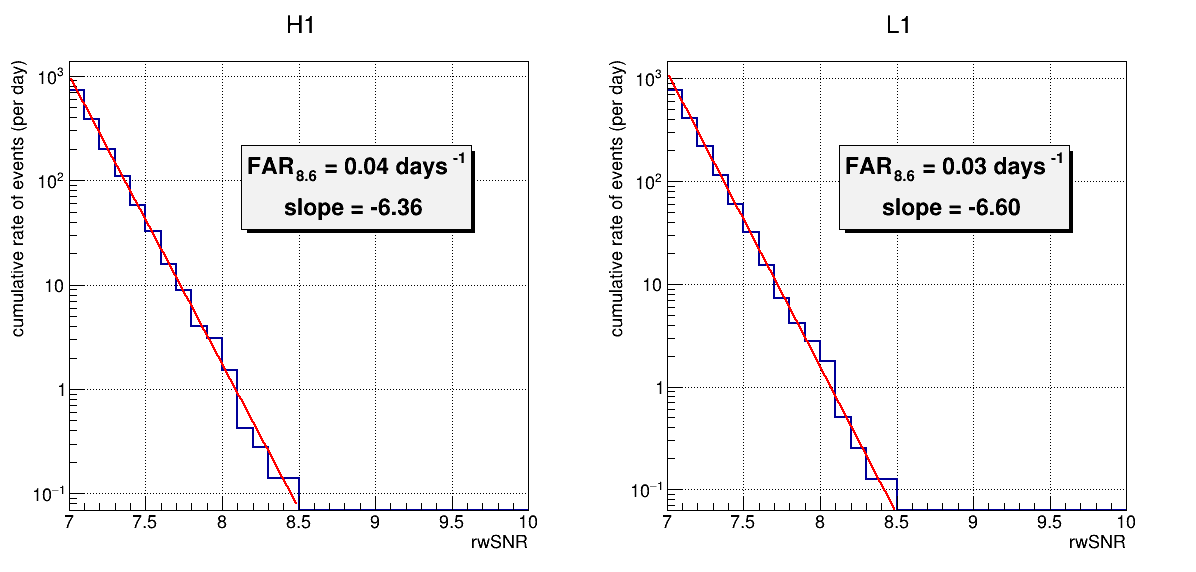
\includegraphics[width=0.9\linewidth]{sectionFAR/simpleFit/cSimpleFit_7_8days.png}
  \end{minipage}
  \hfill
  %
  \begin{minipage}{0.9\linewidth}
    \centering
    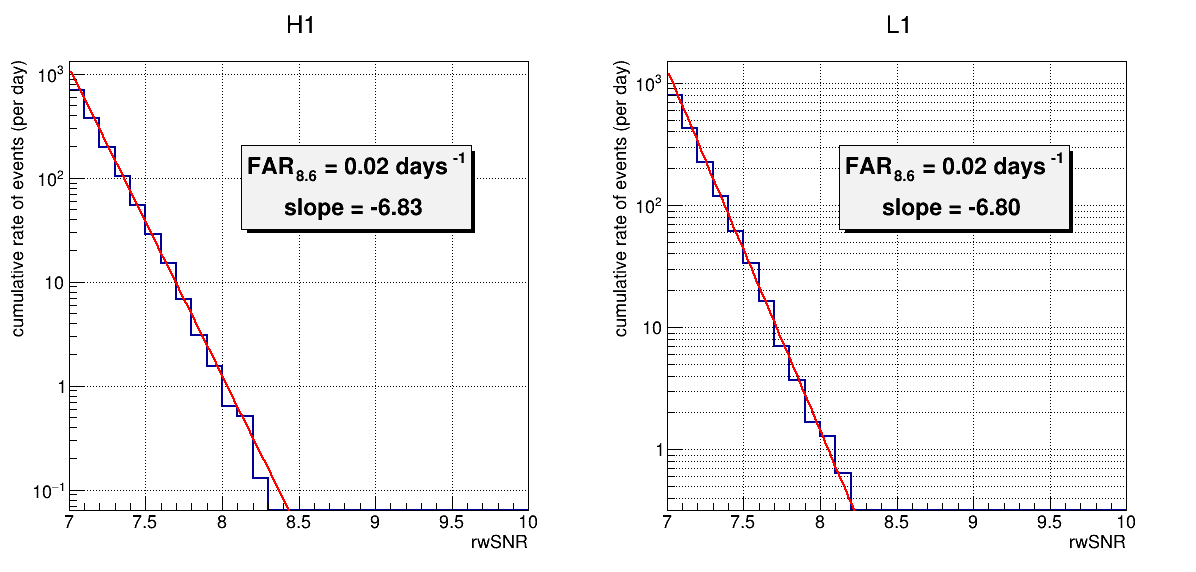
\includegraphics[width=0.9\linewidth]{sectionFAR/simpleFit/cSimpleFit_8_8days.png}
  \end{minipage}
  \hfill
  %
  \begin{minipage}{0.9\linewidth}
    \centering
    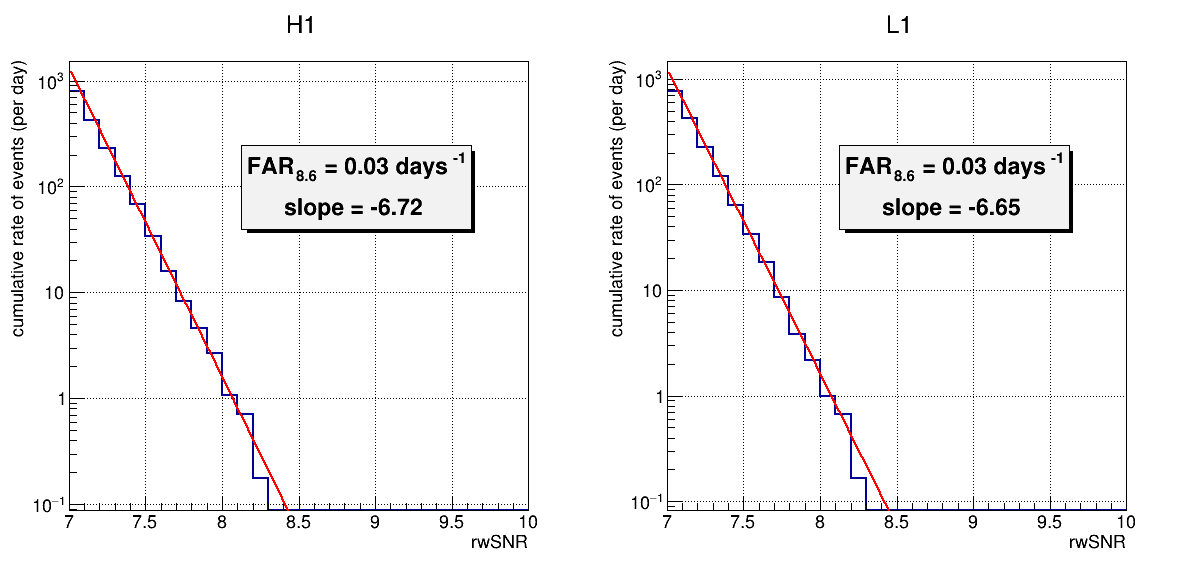
\includegraphics[width=0.9\linewidth]{sectionFAR/simpleFit/cSimpleFit_6_6days.png}
  \end{minipage}
  \hfill
  %
  \caption{rwSNR distribution for EM bright single detector triggers which pass the selection criteria on O3 data analyzed using MBTA O4 configuration. The duty cycles from top to bottom are 7.2, 7.8, 5.7 days for H1 and 7.9, 7.9, 6.0 days for L1. Fit with $\text{FAR$_{8.6}$} \times \exp(\text{slope} \times (\text{rwSNR}-8.6))$.}
  \label{fig:simple_fit}
\end{figure}




%%%%%%%%%%
%\subsection{Background estimation with individual band data}

%\clearpage
\subsection{Combining individual band triggers with random noise}

Fitting the observed background works well when the background does not change much from one day to another.
If, however, the background distribution that we fit has some tail because there was a lot of noise some day, the parametrization will certainly not be reliable.
Furthermore, we are limited to a few days of observation to perform the parametrization if we want for instance to update the background distribution every week or so.
We would therefore like to investigate a method that would estimate the background for FAR below one per few days..

In the case of coincidences, a background distribution is generated by running a coincidence search with time-shifted detector data to ensure any coincidence found is fortuitous.
The FAR corresponding to a given cRS$_0$ is then computed as the rate of background triggers (obtained via these fake coincidences) with cRS larger than cRS$_0$.
We obviously cannot generate a background distribution using time shifted data of several detectors in the case of single detector triggers.
But MBTA allows us to perform a trick to work in a similar way.
The matched-filtering is performed in two separate frequency bands.
In the case of an astrophysical signal we expect the data in the two band to be correlated at adjacent times (figure \ref{fig:chirp}).
We can therefore make an analogy between our two frequency bands and two detectors of the interferometer network.
Taking this analogy as the starting point, we can start working in a similar way as for the coincidence search.
We follow the logic of the single detector trigger constructions which starts by detecting a trigger in one band and combining its MFOs with the available signal in the other band to see if it passes the selection threshold.
%
\begin{figure}[ht]
    \centering
    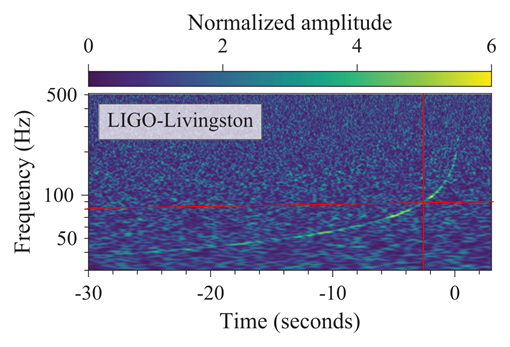
\includegraphics[width=300pt]{sectionFAR/GW170817_chirp.png}
    \caption{GW170817 in the time-frequency plane, extracted and adapted from \cite{gw170817}. The horizontal line shows the limit between the 2 frequency bands defined in MBTA, the vertical line shows the separation in time of the low frequency and high frequency components of the signal. }
    \label{fig:chirp}
\end{figure}
%

Therefore, to emulate this process we need to store single band triggers and single band random noise (random MFOs).
This option is available in the MBTA version prepared for O4 and works as follow:
\begin{itemize}
\item Individual band triggers of each band are saved with an SNR threshold of 5.
  Since there is a very high number of low SNR triggers, they are down-sampled to reduce the computational cost and disk space usage.
  The down-sampling is done between SNR=5 and SNR=9.
  A weight is computed as $w_{ds} = 10^{0.3 \times (9-\text{SNR})}$.
  A random number $r$ is then generated following a uniform distribution, if $r \times w_{ds} \leq 1$ the trigger is saved.
\item MBTA periodically saves random noise in each band for every Real Template (RT, individual band templates),  in general every \SI{2000}{s}$ +\epsilon$ with $\epsilon=\SI{0.11}{s}$.
  This choice is motivated by the fact that FFTs are computed with an integer interval and we could have some edge effects at the time the FFT is computed (such as excess of triggers) although it is unlikely to occur.
  by using an $\epsilon$ we can select our random noise at different time offsets with respect to the time of the computation of the FFT.
  
\end{itemize}
We show in figure \ref{fig:single_band_good} the SNR distribution of the individual band triggers and random noises over two different periods of time (for EM bright templates and times that pass the single detector triggers selection criteria).
We see that we have high rwSNR triggers in the HF band but they constitute at most $\sim 0.1\%$ of the total number of triggers.
Also they will not produce loud noise triggers as we will see, because the \achi and rwSNR step will downgrade them.

We then proceed to make the fake coincidences:
\begin{itemize}
\item The MFOs of the triggers of one band are combined with all random noises of the other band that are associated with a compatible RT.
  The combination is done following
\begin{equation}
  \begin{cases}
    \textrm{MFO}_{\textrm{combi,P}}(t) &= \textrm{MFO}_{\textrm{LF,P}}(t_{LF}) + \cos(\phi)\textrm{MFO}_{\textrm{HF,P}}(t_{HF}) -\sin(\phi)\textrm{MFO}_{\textrm{HF,Q}}(t_{HF})\\
    \textrm{MFO}_{\textrm{combi,Q}}(t) &= \textrm{MFO}_{\textrm{LF,Q}}(t_{LF}) + \sin(\phi)\textrm{MFO}_{\textrm{HF,P}}(t_{HF}) +\cos(\phi)\textrm{MFO}_{\textrm{HF,Q}}(t_{HF})\\
  \end{cases}
\end{equation}
which is the same as for the band MFO combination in MBTA (eq. \ref{eq:mfo_combi}) with the LF part at time $t_{LF}$ and the high frequency part at $t_{HF}$.
The MFO of the low frequency part of the combination (either the trigger or the random noise) first has to be interpolated to account for the difference in sampling rate between the two frequency bands.
Since we have no information about the phase $\phi$, the combination is done for two orthogonal values: $\phi=0$ and $\phi=\pi/2$.

\item The \achi and rwSNR are computed.

\item Repeat with the triggers of the second band and random noise of the first one.
  Note that a small fraction of noise events may come from a trigger in each frequency band.
  In the way we proceed here, this event will be counted as two different events because we have two triggers.
  This means that we have a slight over-estimation and we are therefore being conservative.

\item The effective time for the computed background is
  \begin{equation}
    2 \times \frac{(\textrm{observed effective time})^2}{\textrm{random noise saving period}}
  \end{equation}
  The factor 2 stands for the two phase values used in the combination process.
\end{itemize}
An example of combination of a high frequency trigger with a low frequency random noise is shown in figures \ref{fig:mfo_PQ} and \ref{fig:mfoCombi}.
The rwSNR distribution of the computed background is shown in figure \ref{fig:computed_bkg} using 3.6 days of data in H1 and 6.4 days of data in L1.
The effective time for the computed background is 3.1 years in H1 and 9.7 years in L1.
It is compared to the background observed during the time for which we saved the triggers and random noises, Gaussian noise and O3 background.
We see that we can compute a distribution which follows the observed background, especially at low rwSNR (around 7), without any arbitrairy scaling factor.
However, for larger rwSNR, the computed background is usually below the observed one.

Figure \ref{fig:computed_bkg_cumul} shows the cumulative rate for the computed and observed background.
The computed background is fitted using $\text{FAR$_{8.6}$} \times \exp(\text{slope} \times (\text{rwSNR}-8.6))$.
Fit results are given in table \ref{tab:fitCompBkg}.
The slope in this case is steeper than what we had previously for the observed background in table \ref{tab:simple_fit}.

Figure \ref{fig:computed_splitBand} shows the rwSNR distribution of the computed background split in two: pseudo-events made with a HF trigger and pseudo-events made with a LF trigger.
We see that in H1 the HF band had a greater contribution to the final background but in the case of L1 the contribution of each band is almost equal.

\begin{table}
  \centering
  \resizebox{\linewidth}{!}{%
  \begin{tabular}{c|c|c|c|c|c|c}
    Detector & data duration (days) & FAR$_{8.6}$ (days$^{-1}$) & slope & IFAR$_8$ (days) & IFAR$_9$ (years) & IFAR$_{10}$ (centuries) \\ \hline
    H1 & 3.6 & 0.019 $\pm$ 0.001 & -8.1 $\pm$ 0.1 & 0.34 $\pm$ 0.01 & 3.7 $\pm$ 0.4 & 125 $\pm$ 23 \\
    L1 & 6.4 & 0.042 $\pm$ 0.002 & -7.40 $\pm$ 0.04 & 0.279 $\pm$ 0.005 & 1.26 $\pm$ 0.07 & 20 $\pm$ 2 \\
  \end{tabular}}
  \caption{Parameters of the fits using trigger-random noise coincidences}
  \label{tab:fitCompBkg}
\end{table}


%%%% PLOTS FOR TRIGGERS AND RANDOM NOISES
% FIRST ALL OF THEM
% THEN ONLY EM BRIGHT + NO ER AND GATING

% \begin{figure}[ht]
%   \centering
%   %
%   \begin{minipage}{0.45\linewidth}
%     \centering
%     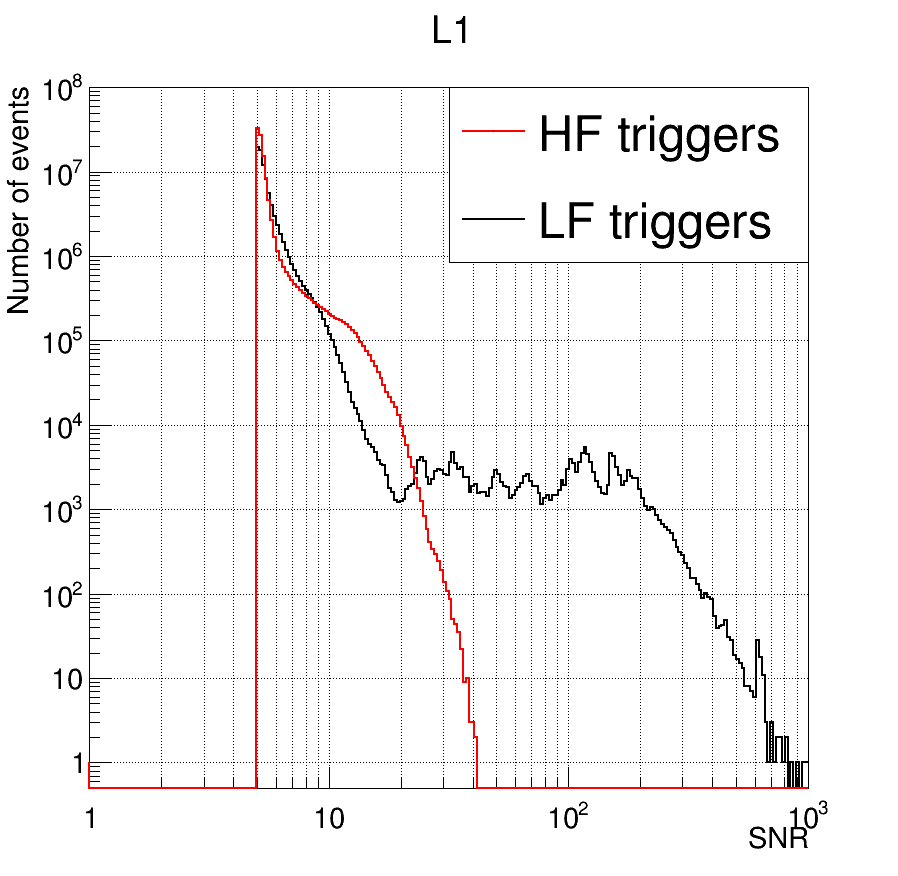
\includegraphics[width=\linewidth]{sectionFAR/O4/cTrig.png}
%     \captionof{figure}{Example of triggers SNR distribution over $\sim 6.34$ days, large tails indicate a noisy period}
%     \label{fig:triggers}
%   \end{minipage}
%   \hfill
%   %
%   \begin{minipage}{0.45\linewidth}
%     \centering
%     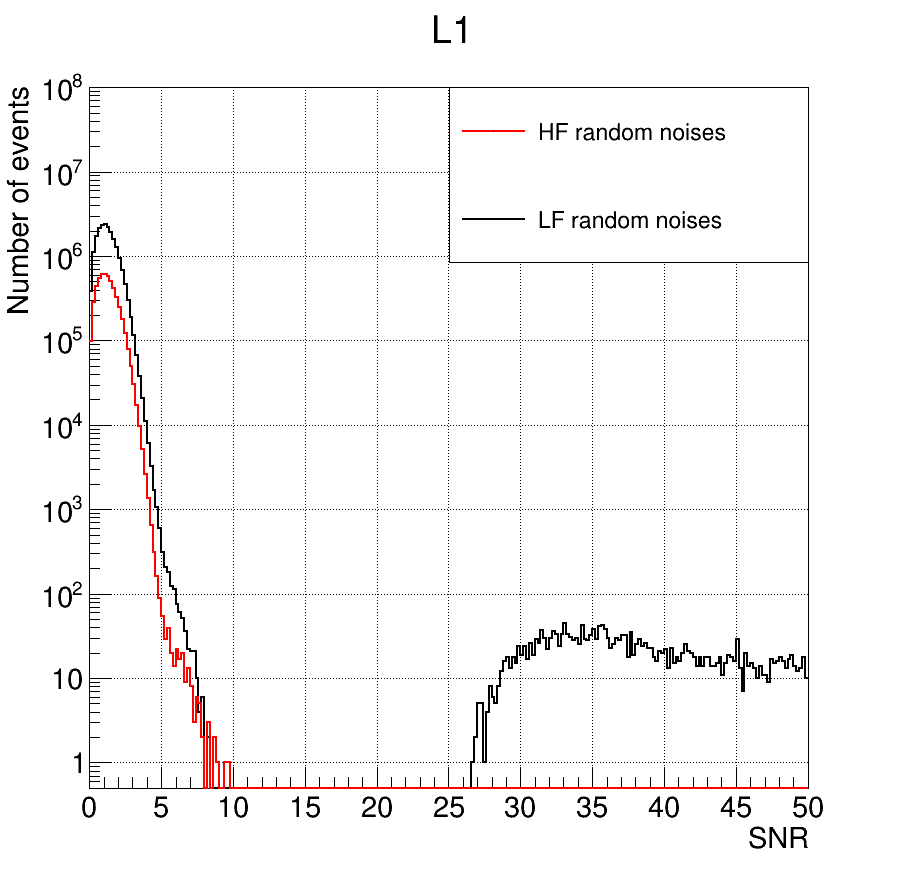
\includegraphics[width=\linewidth]{sectionFAR/O4/cRand.png}
%     \captionof{figure}{Example of random noises SNR distribution over $\sim 6.34$ days}
%     \label{fig:randoms}
%   \end{minipage}
%   \hfill
% \end{figure}




\begin{figure}[ht]
  \centering
  %
  \begin{minipage}{0.45\linewidth}
    \centering
    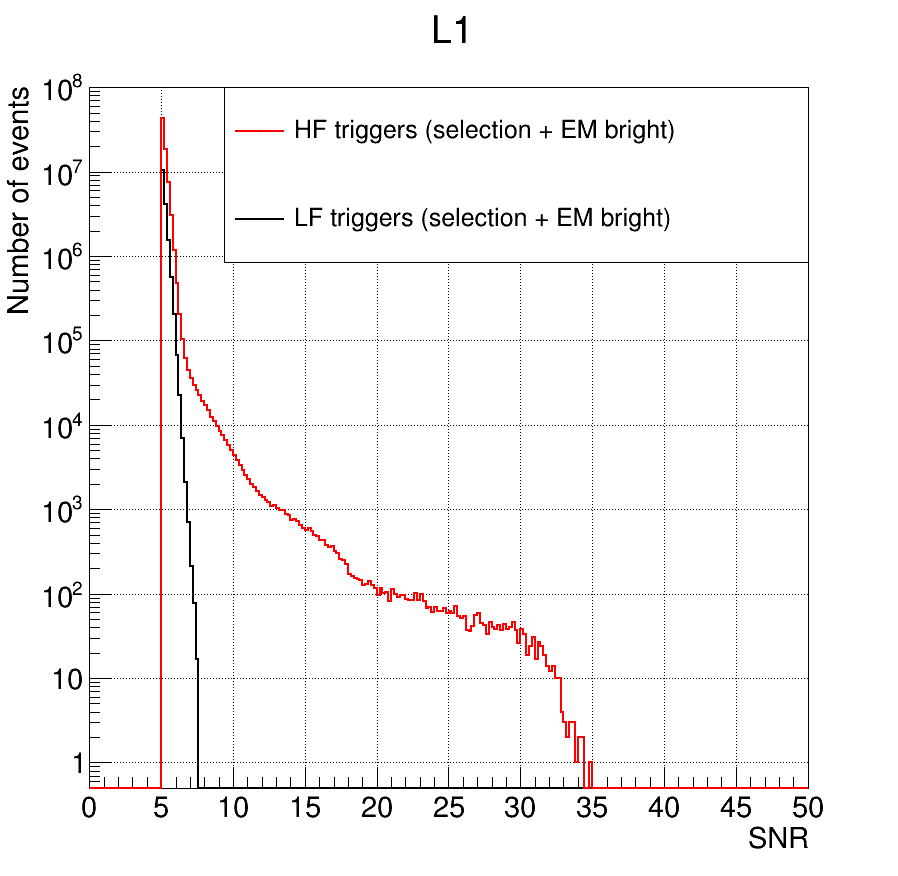
\includegraphics[width=\linewidth]{sectionFAR/O4/cTrig_good_730000.png}
  \end{minipage}
  \hfill
  %
  \begin{minipage}{0.45\linewidth}
    \centering
    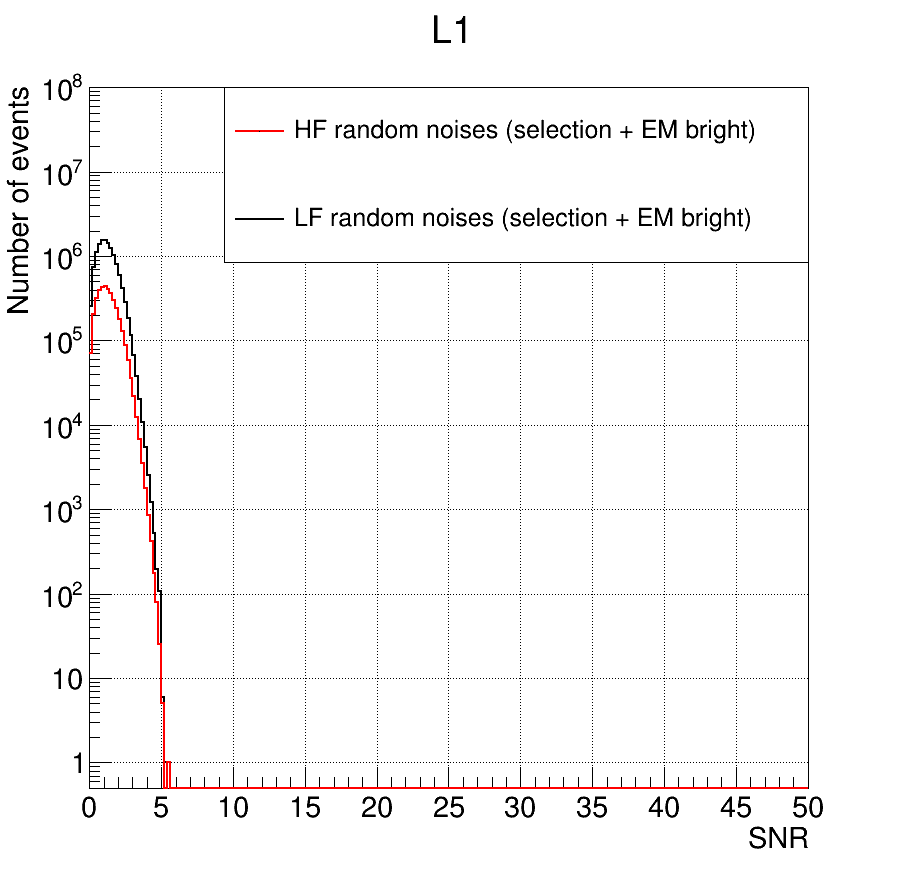
\includegraphics[width=\linewidth]{sectionFAR/O4/cRand_good_730000.png}
  \end{minipage}
  % 
  \begin{minipage}{0.45\linewidth}
    \centering
    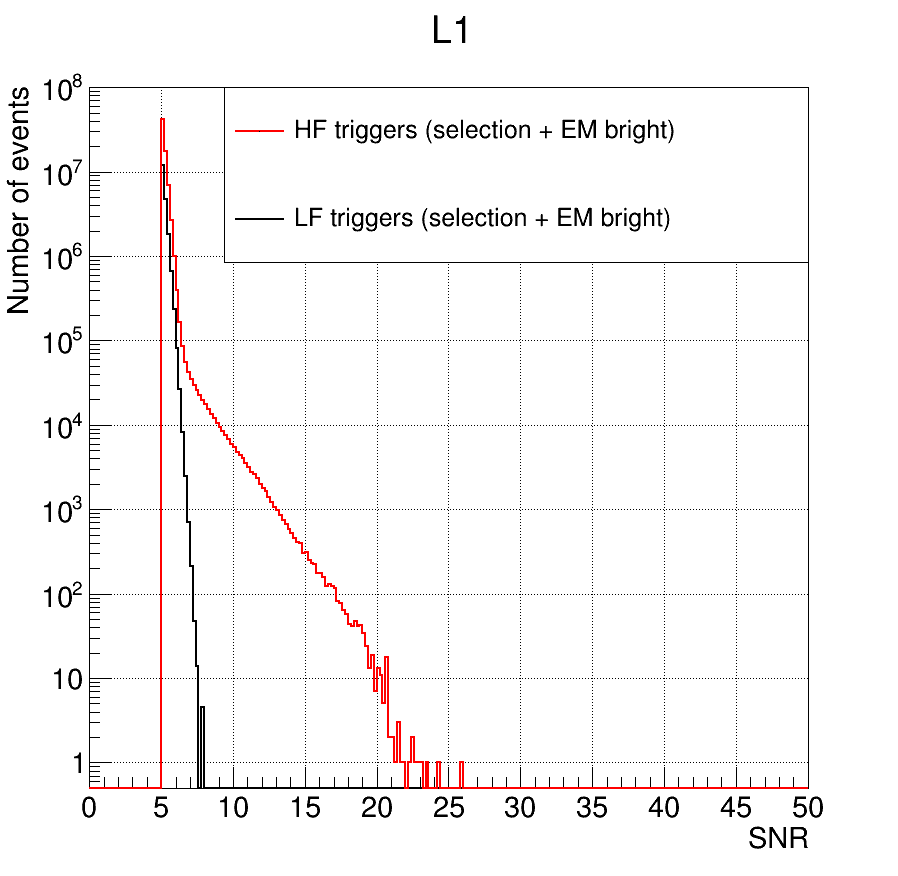
\includegraphics[width=\linewidth]{sectionFAR/O4/cTrig_good.png}
  \end{minipage}
  \hfill
  %
  \begin{minipage}{0.45\linewidth}
    \centering
    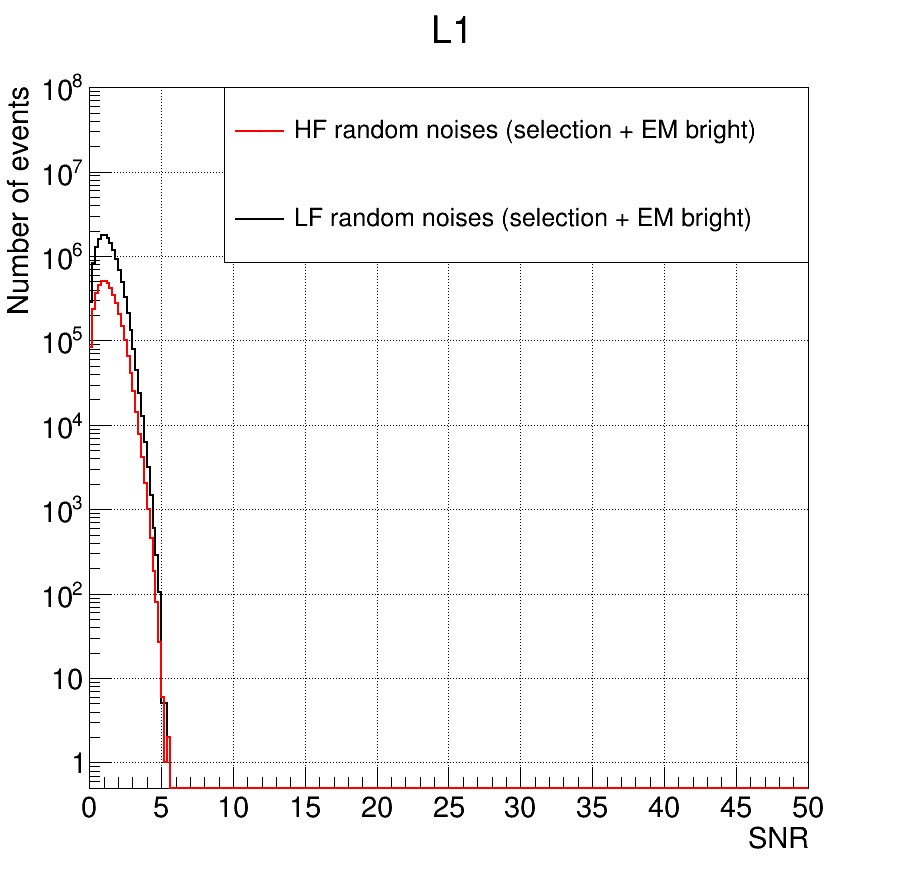
\includegraphics[width=\linewidth]{sectionFAR/O4/cRand_good.png}
  \end{minipage}
  \hfill
  \caption{Example of triggers (left) and random noise (right) SNR distribution over effective $\sim 6.4$ days (top, from February 12 2023 to February 24 2023) and $\sim 6.34$ days (bottom, from February 28 2023 to March 10 2023) in L1, only for EM bright with single selection criteria applied.
    The downsampling weights of the triggers are taken into account.
    The 6.4 days are the same ones as those used for the computation of the background in L1 presented in this chapter.}
  \label{fig:single_band_good}
\end{figure}





%%%%% PLOTS MFO P ET Q TRIGGER, RANDOM, COMBINED


\begin{figure}[ht]
    \centering
    \begin{minipage}{\linewidth}
        \centering
        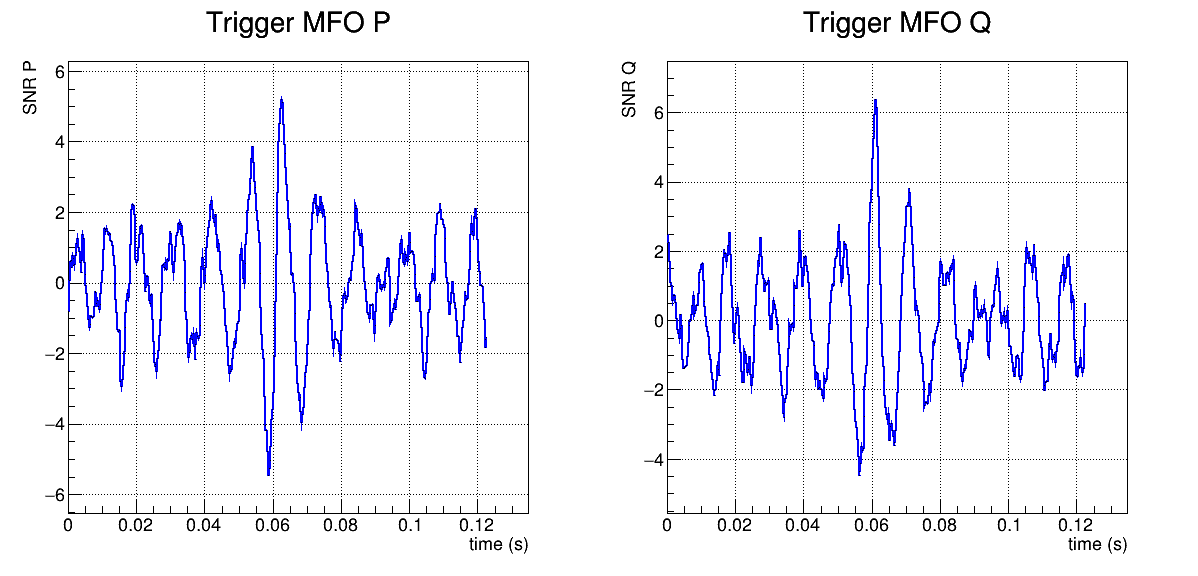
\includegraphics[width=0.8\linewidth]{sectionFAR/O4/cTrigMFO.png}
    \end{minipage}
    \hfill
    %
    \begin{minipage}{\linewidth}
        \centering
        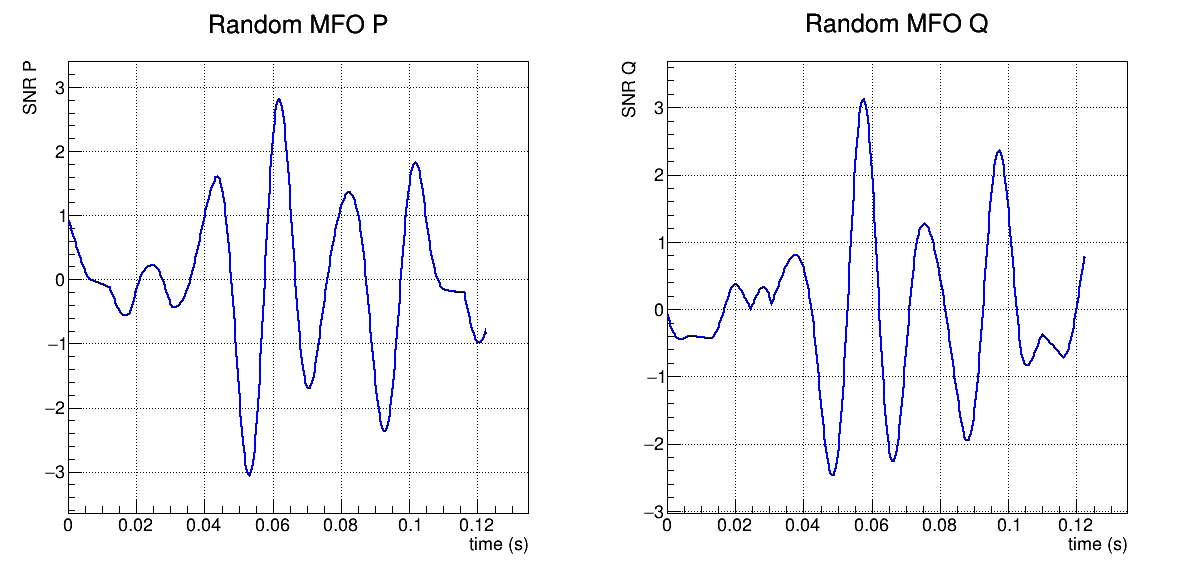
\includegraphics[width=0.8\linewidth]{sectionFAR/O4/cRandMFO.png}
    \end{minipage}
    \hfill
    \vspace{5mm}
    %
    \begin{minipage}{\linewidth}
        \centering
        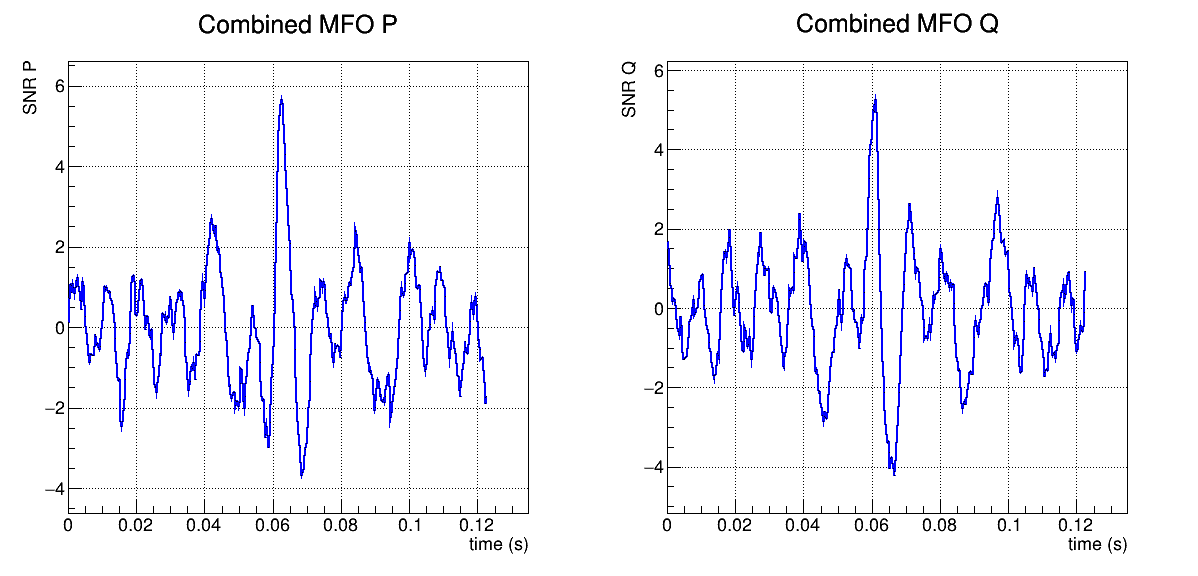
\includegraphics[width=0.8\linewidth]{sectionFAR/O4/cCombiMFO.png}
    \end{minipage}
    \hfill
    \caption{Top: P and Q MFOs for a HF trigger in L1. Middle: P and Q MFOs for a LF random noise in L1. Bottom: In-phase and in-quadrature SNR time series for the event resulting from the combination of the two. Mind the differences in Y-axis range.}
    \label{fig:mfo_PQ}
\end{figure}

\begin{figure}
  \centering
  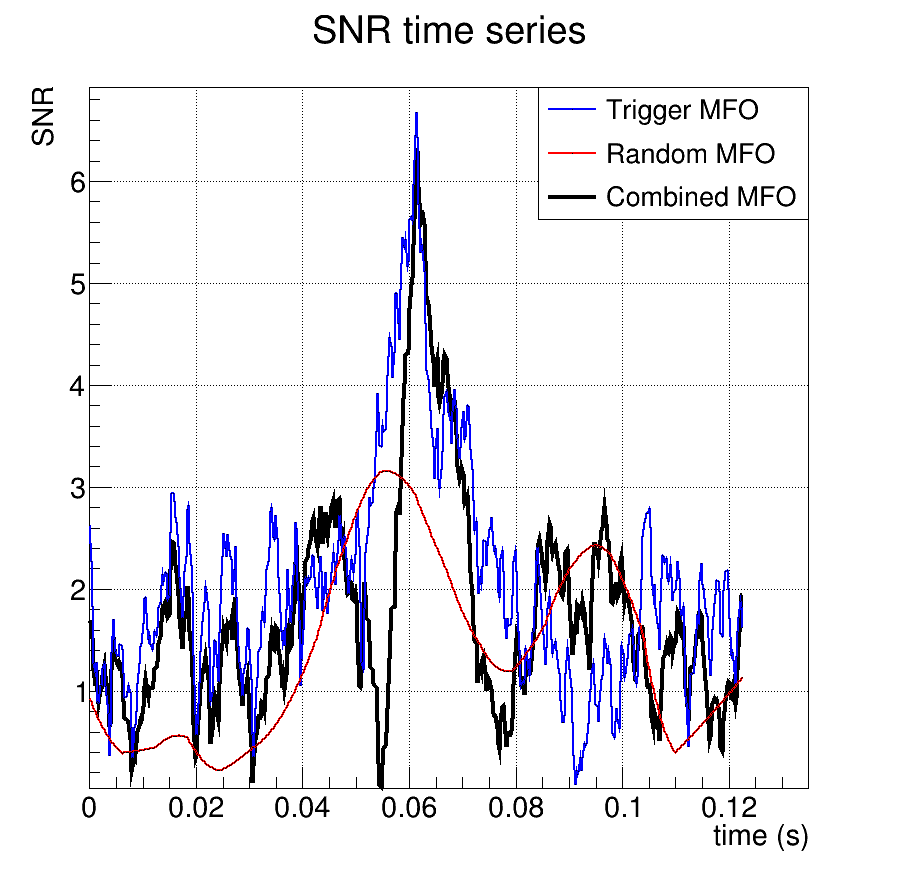
\includegraphics[width=0.5\linewidth]{sectionFAR/O4/cSnrMFO.png}
  \captionof{figure}{SNR time series for the trigger, random noise and pseudo-event resulting from the combination of the trigger and random MFO show in figure \ref{fig:mfo_PQ}}
  \label{fig:mfoCombi}
\end{figure}


%%%% PLOT FOR COMBINED EVENTS, EM BRIGHT + NO ER AND GATING

% \begin{figure}
%   \centering
%   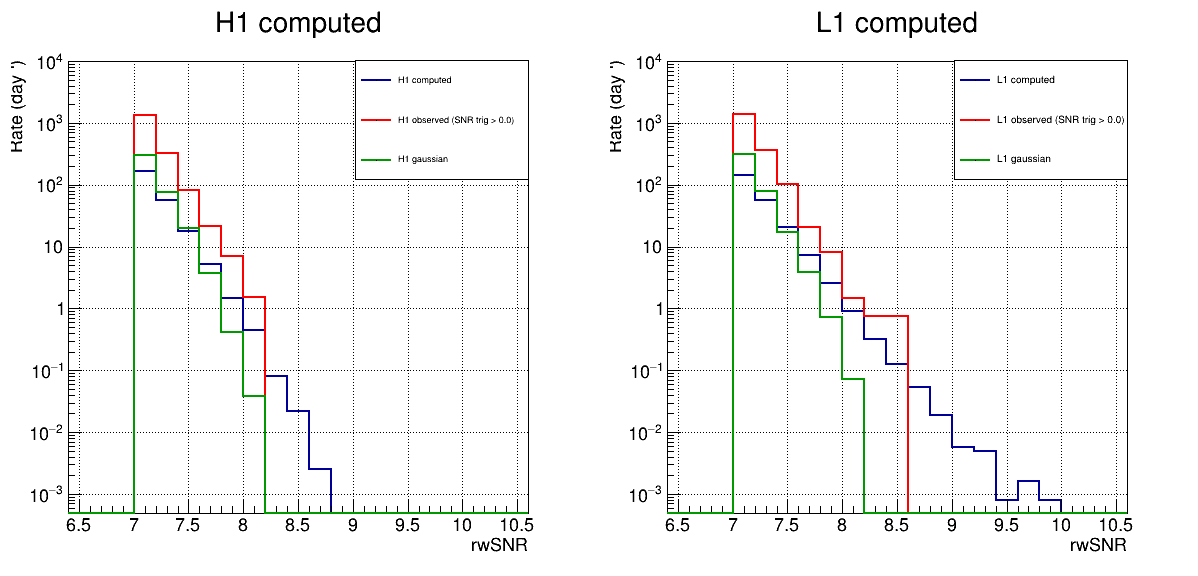
\includegraphics[width=\linewidth]{sectionFAR/O4/cNew.png}
%   \caption{Comparison of the computed background with the observed background and simulated gaussian noise. The observed background is for the same time range as the triggers and random noises used to compute the background. EM bright only and single selection is applied. \textcolor{red}{Retirer ce plot et ne garder que le suivant ?}}
%   \label{fig:computed_bkg}
% \end{figure}


\begin{figure}
  \centering
  \begin{minipage}{0.45\linewidth}
    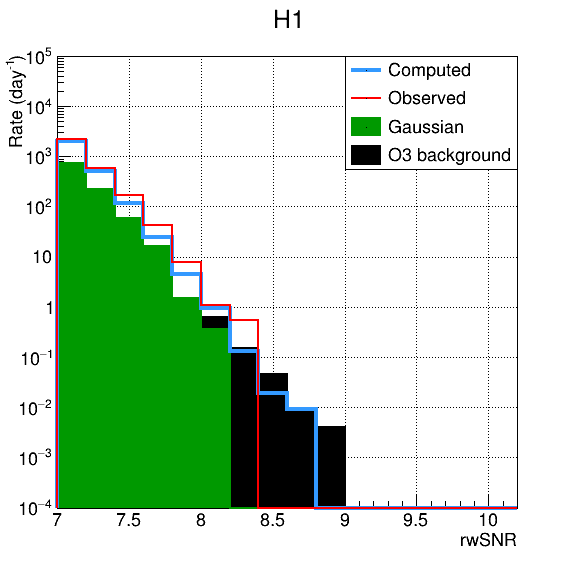
\includegraphics[width=\linewidth]{sectionFAR/O4/cComputedH1.png}
  \end{minipage}
  %
  \begin{minipage}{0.45\linewidth}
    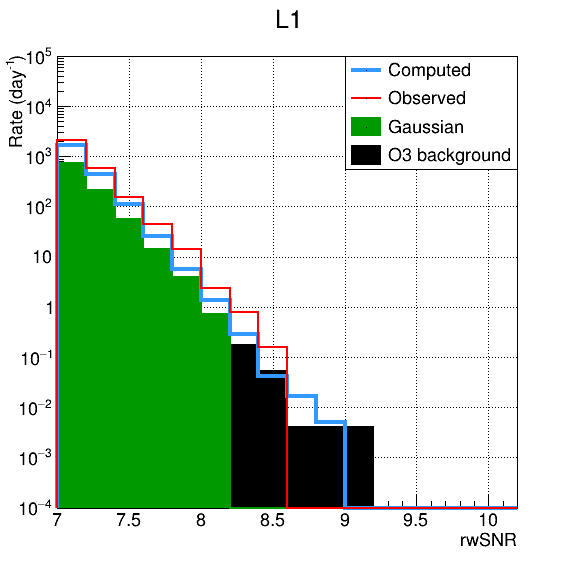
\includegraphics[width=\linewidth]{sectionFAR/O4/cComputedL1.png}
  \end{minipage}
  \caption{Comparison of the non-cumulative rate of computed background (blue, trigger-random noise coincidences) with the background observed during the time used for the computation (red), simulated gaussian noise (green, for around one month of data) and all-O3 background (black).
    Left is for 3.6 days of data in H1.
    Right is for 6.4 days of data in L1.
    The ``observed background'' is O3 data analyzed with MBTA O4 configuration as opposed to O3 background which was analyzed with the O3 configuration.
    We only consider triggers from the EM bright region which passed the single selection.}
  \label{fig:computed_bkg}
\end{figure}


\begin{figure}
  \centering
  \begin{minipage}{0.45\linewidth}
    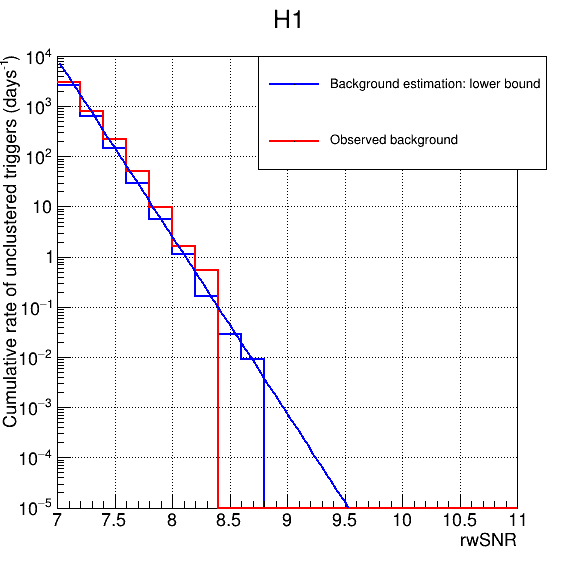
\includegraphics[width=\linewidth]{sectionFAR/O4/cRateCompCumulH1_380000.png}
  \end{minipage}
  %
  \begin{minipage}{0.45\linewidth}
    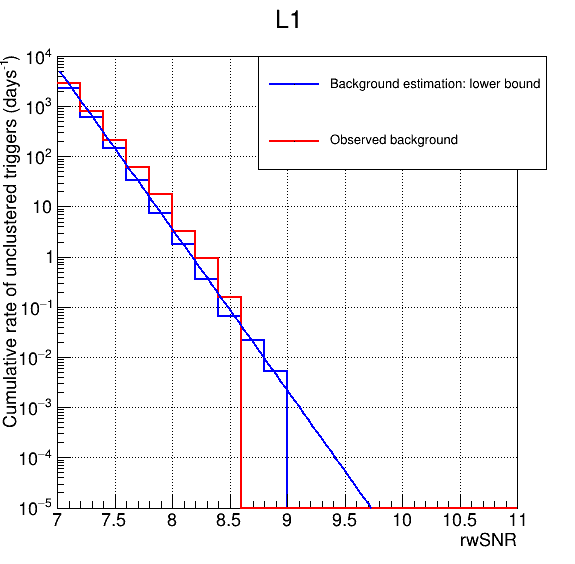
\includegraphics[width=\linewidth]{sectionFAR/O4/cRateCompCumulL1_730000.png}
  \end{minipage}
  \caption{Cumulative rate for the computed background (blue) and observed background (red) shown in figure \ref{fig:computed_bkg}.
    Left is for 3.6 days of data in H1.
    Right is for 6.4 days of data in L1.}
  \label{fig:computed_bkg_cumul}
\end{figure}




\begin{figure}
  \centering
  \begin{minipage}{0.45\linewidth}
    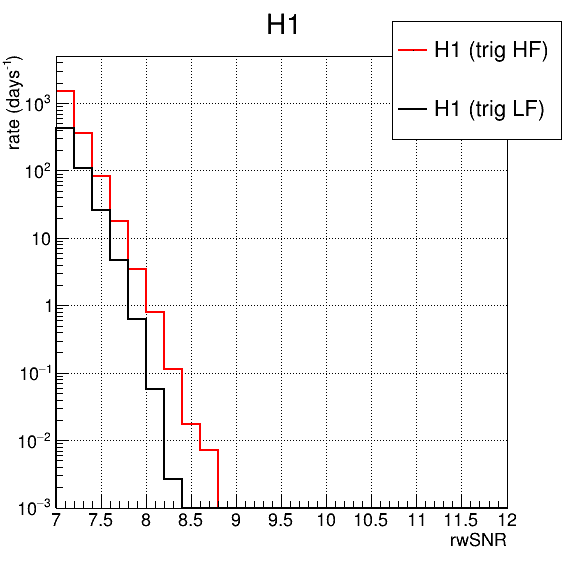
\includegraphics[width=\linewidth]{sectionFAR/O4/cRwSplitTrigH1_380000.png}
  \end{minipage}
  \begin{minipage}{0.45\linewidth}
    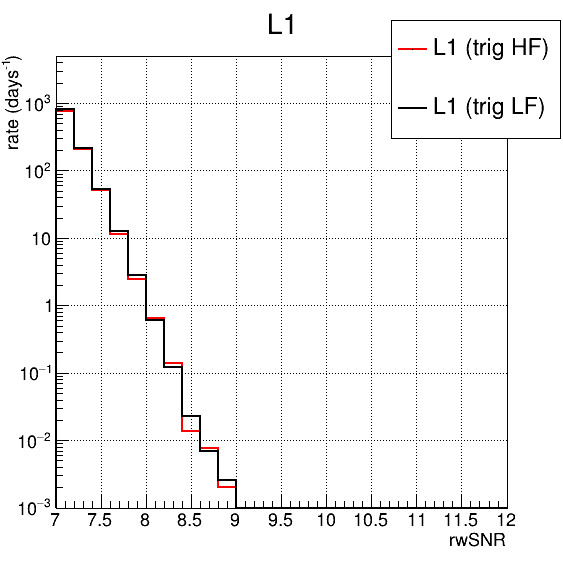
\includegraphics[width=\linewidth]{sectionFAR/O4/cRwSplitTrigL1_730000.png}
  \end{minipage}
  \caption{Computed background rwSNR distribution for 3.6 days in H1 (left) and 6.4 days in L1 (right) using trigger-random noise coincidences separated based on the frequency band of the trigger.
  Red is for pseudo-events made with a HF trigger. Black is for those made with a LF trigger.}
  \label{fig:computed_splitBand}
\end{figure}


%%%%%%%%%%
\clearpage
\subsection{Combining individual bands triggers with other triggers}

We have until now only considered triggers-random noises associations.
This means that we assumed our frequency bands to be completely uncorrelated.
But what if, for example, a glitch occurs at the time the signal changes frequency bands, and therefore could pollute both MBTA's frequency bands?
Then our single detector trigger will likely be formed from two single band triggers, implying some correlation between our bands.
We will therefore also consider trigger-trigger concidences when esimating our background.
This way we can have anything between fully correlated frequency bands (100\% trigger-trigger coincidences) and completely uncorrelated bands (100\% trigger-random noise coincidences).

We will proceed in the same way as for the coincidences with random noise but we have to be careful about two things:
\begin{itemize}
\item triggers were not saved periodically as random noises were, meaning that we do not have a fix number of them for each template.
  In order to easily scale the computed distribution to a rate comparable to the observed background we decide to do a fixed number of coincidences for each template.
  To account for the down-sampling we have to use the down-sampling weight of the second trigger (the one which takes the place of the random noise in the previous section) when counting the number of coincidences we make.
\item triggers were down-sampled unlinke random noises, we have to take this into account when building the distributions (rwSNR distribution for instance) for the pseudo-events.
  Thus, a pseudo-event made from a trigger-trigger combination will have count equal to the product of the downsampling weights of the two triggers.
\end{itemize}
For example combining a trigger from the first band with two triggers from the other band, one with a weight of 3.4 and the other of 1, will count as a total of 4.4 coincidences.
Then when building distributions we will count the coincidences as the product of the down-sampling weight of the first and second trigger.
So in the previous case if the first trigger had a weight of, say 2.1, our first fake single detector trigger would count as $2.1 \times 3.4 = 7.14$ and the second one as $2.1 \times 4.4 = 9.24$.
Regarding the number of coincidences that we want to make, as explained in the first point, it is quite arbitrary although constrained by the quantity of data available or that we want to analyze: the more coincidences the better (computing time aside) but we have to have enough triggers for that.
We want to at least reach the threshold for public alerts.
This means that the computed background should be given for an effective time of at least one year.
Since we typically consider close to a week of data to make the fake coincidences, this can be achieved by doing around 100 coincidences per trigger.
But our goal is also to give high rwSNR trigger a FAR that reflects properly their significance.
Using 1000 coincidences allows to reach FARs of around 1 per 33 years when using 6 days of effective data before even extrapolating.
Thus we choose to do 1000 coincidences per triggers.

If we have enough triggers in each band to make 1000 coincidences per trigger, then we can use any of the two to pick primary triggers and the other to pick secondary triggers (playing the role of the random noise in the previous section).
In case not enough coincidences could be made for a given real template, we decide to use the adjacent ones (RT index-1 and RT index+1) to compensate.
This has also prompted us to use LF triggers as secondary triggers and the HF triggers as primary triggers, since LF RTs should be very similar for adjacent templates.

To summarize:
\begin{itemize}
\item Consider one HF trigger with down-sampling weight $\omega_{\textrm{HF}}$.
\item The real template of this HF trigger is compatible with one or several LF RTs.
\item Let's take the first LF RT which has index $k$ and all associated triggers.
\item Let $N$ be the number of such LF triggers, each of them has a down-sampling weight $\omega_i$ with $i\in \left[|1;N\right|]$.
\item We want to make 1000 fake coincidences, this means that if $N>1000$ we will in fact only use the first $n<N$ LF triggers such that
  \begin{equation}
    \sum_{i=1}^{n-1}\omega_i < 1000 \leq \sum_{i=1}^{n}\omega_i
  \end{equation}

\item If $N<1000$ the relation still holds, simply some of the triggers will have index $k-1$ and/or $k+1$ (although we cannot exclude that for a very small number of templates it may not be possible to gather enough triggers).
\item When counting coincidences, each of those coincidences will count as $\omega_{\textrm{HF}} \times \omega_i$.
\item Since we have effectively done (close to) 1000 coincidences, we can scale the computed distribution with
  \begin{equation}
    T_{\textrm{eff}} = T_{\textrm{eff,ini}} \times 2 \times 1000
  \end{equation}
  where $T_{\textrm{eff,ini}}$ is the initial effective time of the data we use to make the fake coincidences and the factor 2 comes from the two values we use for the phase like with the random noises.
\end{itemize}

Proceeding in this way leads us to a very large over-estimation of the background since it assumes that all triggers in one band are connected to a trigger in the other band.
In order to have a background estimation that can act as an upper bound we choose to scale the distribution computed with trigger-trigger coincidences to force an equal rate with the observed background for a rwSNR of $7.5$, the scaling factor is in this case around $10^{-4}$.
We chose to scale at rwSNR=7.5 as it is a bin with many pseudo-events, meaning reduced errors and also beceause at lower rwSNR we observe a threshold effect due to the selection of triggers starting at SNR=5.
While completely ad hoc this allows us to have an estimation of the background rate close to the observed one and a less steep slope.
Results are shown in figure \ref{fig:computed_rate}.
Note that for H1, due to the smaller observing time used for the computation, only 100 coincidences per trigger were done.
This upper bound estimation is safer in terms of FAR computation because it will lead us to over-estimate the FAR (whereas the lower bound would lead to an under-estimation) and therefore we are less likely to claim false detections since the lower the FAR the more significant the event.
Like for trigger-random noise coincidences, the computed background using trigger-trigger combinations follows an exponential shape.
We can thus go further and extrapolate the computed distribution (actually the cumulative distribution of the computed background) with an exponential function to reach even lower values of FAR as shown in figures \ref{fig:computed_rate_cumul}. Results of the fit for several background estimations are given in table \ref{tab:fit_far}.
These background parametrization can be done in terms of cRS$^2$ in order to be used by the p$_{\textrm{astro}}$ code to compute in the end a FAR(p$_{\textrm{astro}}$).

In all this chapter we have computed this background using different methods.
It should be higlighted that in all cases the background distribution could be fitted with an exponential function with the same slope over the full rwSNR range.
This gives us confidence in the background extrapolation we can do to reach lower FAR.

%
% \begin{table}[h]
%   \centering
%   \begin{tabular}{c|c|c|c|c}
%     Detector & data duration used for estimation & constant & slope & rwSNR(1 per 10 months) \\ \hline
%     H1 & 3.7 days & 64.8 $\pm$ 3.1 & -7.78 $\pm$ 0.36 & 9.06 \\ \hline
%     L1 & 3.7 days & 66.3 $\pm$ 1.3 & -7.94 $\pm$ 0.15 & 9.07 \\ \hline
%     L1 & 6.4 days & 56.6 $\pm$ 0.5 & -6.69 $\pm$ 0.06 & 9.32 \\ \hline
%     L1 & 3.61 days & 66.7 $\pm$ 1.4 & -7.99 $\pm$ 0.17 & 9.06 \\ \hline
%     L1 & 3.54 days & 60.7 $\pm$ 0.6 & -7.22 $\pm$ 0.07 & 9.20 \\
%   \end{tabular}
%   \caption{Results of the fits performed on the computed over-estimation of the background for different detectors and duration. Fit function is $\exp( \textrm{constant} + \textrm{slope} \times \textrm{rwSNR})$.}
%   \label{tab:fit_far}
% \end{table}

%
\begin{table}[h]
  \centering
  \resizebox{\linewidth}{!}{%
  \begin{tabular}{c|c|c|c|c|c|c}
    %Detector & fit range & FAR$_8$ (days$^{-1}$) & slope & IFAR$_9$ (days) & IFAR$_{10}$ (years) \\ \hline
    %H1 & 3.6 days & 11.57 $\pm$ 1.08 & -7.77 $\pm$ 0.17 &  & 2.05e-06 $\pm$ 6.98e-07 \\ 
    %H1 & 3.7 days & 14.01 $\pm$ 1.13 & -7.78 $\pm$ 0.14 &  & 2.47e-06 $\pm$ 1.00e-06 \\ 
    %L1 & 6.4 days & 23.09 $\pm$ 0.96 & -6.69 $\pm$ 0.07 &  & 3.60e-05 $\pm$ 4.12e-06 \\ 
    %L1 & 3.8 days & 17.47 $\pm$ 1.33 & -7.94 $\pm$ 0.14 &  & 2.22e-06 $\pm$ 8.54e-07 \\ 
    %L1 & 3.6 days & 14.85 $\pm$ 1.26 & -7.99 $\pm$ 0.15 &  & 1.69e-06 $\pm$ 7.25e-07 \\
    %L1 & 3.5 days & 18.53 $\pm$ 0.44 & -7.22 $\pm$ 0.04 &  & 9.84e-06 $\pm$ 2.79e-06 \\
    %
    %H1 & 3.6 days & 11.6 $\pm$ 1.1 & -7.8 $\pm$ 0.2 & 205.4 $\pm$ 22.2 & 1337.7 $\pm$ 455.9 \\ 
    %H1 & 3.7 days & 14.0 $\pm$ 1.1 & -7.8 $\pm$ 0.1 & 170.0 $\pm$ 15.9 & 1109.6 $\pm$ 325.1 \\ 
    %L1 & 6.4 days & 23.1 $\pm$ 1.0 & -6.7 $\pm$ 0.1 & 34.7 $\pm$ 1.3 & 76.2 $\pm$ 8.7 \\ 
    %L1 & 3.8 days & 17.5 $\pm$ 1.3 & -7.9 $\pm$ 0.1 & 160.6 $\pm$ 11.4 & 1234.9 $\pm$ 274.5 \\ 
    %L1 & 3.6 days & 14.9 $\pm$ 1.3 & -8.0 $\pm$ 0.2 & 199.6 $\pm$ 15.8 & 1619.9 $\pm$ 400.7 \\
    %L1 & 3.5 days & 18.5 $\pm$ 0.4 & -7.2 $\pm$ 0.0 & 74.1 $\pm$ 3.8 & 278.4 $\pm$ 45.6 \\
    Detector & data duration (days) & FAR$_{8.6}$ (days$^{-1}$) & slope & IFAR$_8$ (days) & IFAR$_9$ (years) & IFAR$_{10}$ (centuries) \\ \hline
    H1 & 3.6 & 0.109 $\pm$ 0.001 & -7.8 $\pm$ 0.1 & 0.087 $\pm$ 0.003 & 0.56 $\pm$ 0.02 & 13.1 $\pm$ 1.2 \\
    H1 & 3.7 & 0.132 $\pm$ 0.002 & -7.8 $\pm$ 0.1 & 0.069 $\pm$ 0.004 & 0.48 $\pm$ 0.02 & 11.9 $\pm$ 1.8 \\
    L1 & 6.4 & 0.418 $\pm$ 0.003 & -6.70 $\pm$ 0.04 & 0.043 $\pm$ 0.001 & 0.096 $\pm$ 0.002 & 0.8 $\pm$ 0.1 \\
    L1 & 3.5 & 0.243 $\pm$ 0.001 & -7.24 $\pm$ 0.04 & 0.053 $\pm$ 0.001 & 0.205 $\pm$ 0.004 & 2.9 $\pm$ 0.2 \\
    L1 & 3.6 & 0.122 $\pm$ 0.002 & -8.1 $\pm$ 0.1 & 0.065 $\pm$ 0.005 & 0.56 $\pm$ 0.03 & 17.8 $\pm$ 3.2 \\
    L1 & 3.8 & 0.149 $\pm$ 0.003 & -8.0 $\pm$ 0.1 & 0.055 $\pm$ 0.004 & 0.45 $\pm$ 0.03 & 13.6 $\pm$ 2.4 \\
  \end{tabular}}
  \caption{Results of the fits performed on the computed over-estimation of the background for different detectors and times. Fit function is $\textrm{FAR$_{8.6}$} \times \exp(\textrm{slope}(\textrm{rwSNR}-8.6))$.}
  \label{tab:fit_far}
\end{table}


\begin{figure}
  \centering
  \begin{minipage}{0.45\linewidth}
    \centering
    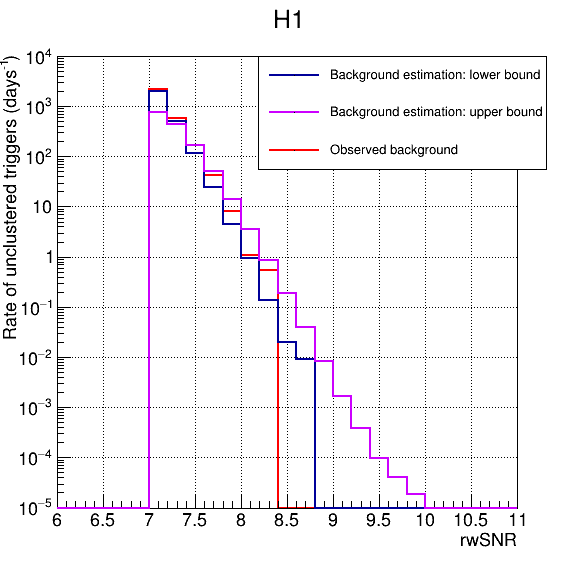
\includegraphics[width=\linewidth]{sectionFAR/O4/cRateH1.png}
  \end{minipage}
  \hfill
  % 
  \begin{minipage}{0.45\linewidth}
    \centering
    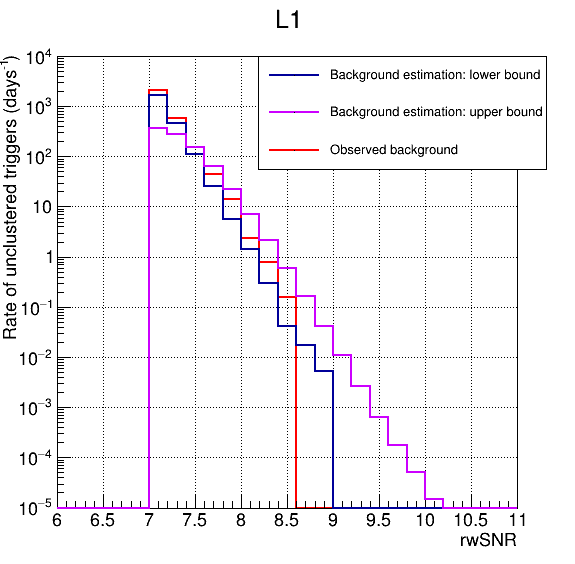
\includegraphics[width=\linewidth]{sectionFAR/O4/cRateL1.png}
  \end{minipage}
  \hfill
  \caption{Comparison of the non-cumulative rate for the computed lower bound, upper bound and observed background for H1 (left) and L1 (right). Computation was done over $\sim 3.6$ and $\sim 6.4$ days for H1 and L1 respectively.}
  \label{fig:computed_rate}
\end{figure}


\begin{figure}
  \centering
  \begin{minipage}{0.45\linewidth}
    \centering
    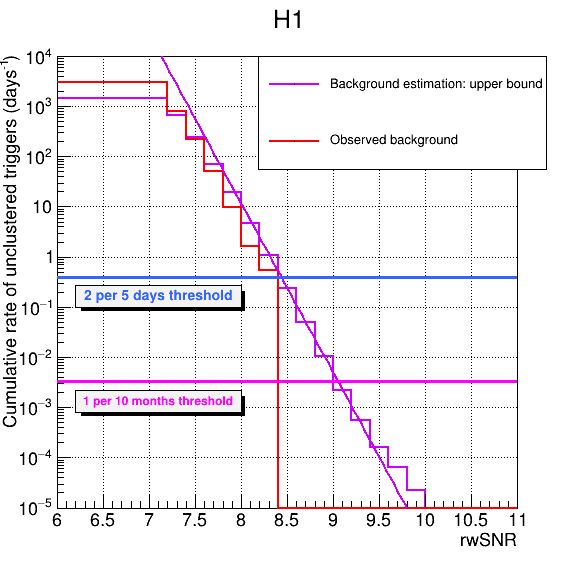
\includegraphics[width=\linewidth]{sectionFAR/O4/cRateCumulH1.png}
  \end{minipage}
  \hfill
  % 
  \begin{minipage}{0.45\linewidth}
    \centering
    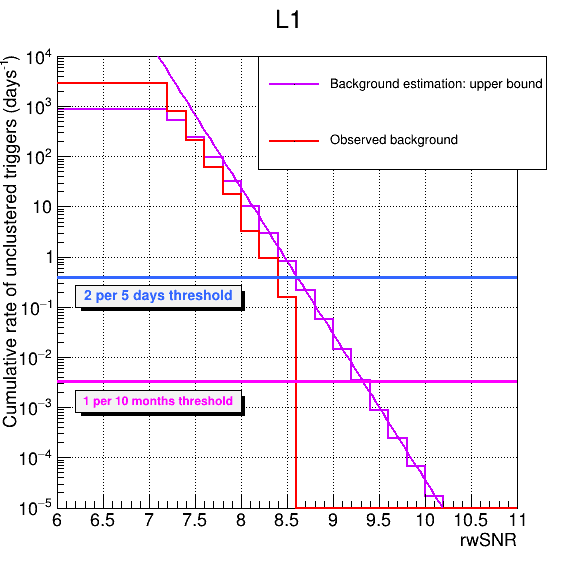
\includegraphics[width=\linewidth]{sectionFAR/O4/cRateCumulL1.png}
  \end{minipage}
  \hfill
  \caption{Comparison of the cumulative distributions of the observed background and computed upper bound for the background in H1 (left, for $\sim 3.6$ days of data) and L1 (right, for $\sim 6.4$ days of data) fitted with an exponential function. Fit results are given in table \ref{tab:fit_far}.
  Horizontal lines show the FAR thresholds used to send low-significance (2 per 5 days) and significant (1 per 10 months) public alerts at the begining of O4.}
  \label{fig:computed_rate_cumul}
\end{figure}
